\chapter*{Preface}
\addcontentsline{toc}{chapter}{Preface}

\section*{Organization}

The chapters of this thesis have been written so that they could mainly
be read independently from one another.

The introduction (\Cref{ch:intro}) is targeted at anyone with
a reasonable understanding of theoretical computer science---corresponding roughly
to a master's level. This chapter is not technical and introduces as few definitions
as possible. Its goal is to provide an overview of the foundational results of the
field, the questions we studied in this thesis, our contributions, as well
as the most important open questions that remain to be solved.
\textbf{If you should only read one chapter of this thesis, let it be \Cref{ch:intro}!}

The next chapter presents the general preliminaries (\Cref{ch:general-preliminaries}):
it serves no other purpose but to make all notions unambiguous. We advise
the reader to quickly skim over it, and to go back to this chapter only when
needed.

This thesis is then divided in two independent parts:
the first one focuses on database theory (\Cref{part:databases}),
and the second one on automatic structures (\Cref{part:automatic}).
Each part starts with a quick survey of the domain
(\Cref{ch:prelim-graph-databases,ch:preliminaries-automatic-structures}),
followed by two chapters presenting our main contributions in this domain
(\Cref{ch:minimization-CRPQ,ch:semantic-tree-width-CRPQ} for database theory,
and \Cref{ch:dichotomy-theorem,ch:algebra} for automatic structures).
Finally, each part is concluded by a discussion (\Cref{ch:conclu-database,ch:conclu-automatic}),
mostly about open problems, but also on techniques that we used to attempt (and failed) to solve these problems.

A succinct global table of content is presented in \Cref{sec:contents},
and each chapter is preceded by a more detailed one.
\begin{marginfigure}
	\centering
	\begin{tikzpicture}
		\node at (-1,0) (1) {\ref{ch:intro}};
		\node at (1,0) (2) {\ref{ch:general-preliminaries}};
		\node[below=1.5cm of 1] (3) {\ref{ch:prelim-graph-databases}};
		\node[below left=1.5cm and 1cm of 3] (4) {\ref{ch:minimization-CRPQ}};
		\node[below right=1.5cm and 1cm of 3] (5) {\ref{ch:semantic-tree-width-CRPQ}};
		\node[below left=1.5cm and 1cm of 5] (6) {\ref{ch:conclu-database}};
		\node[below=1.5cm of 2] (7) {\ref{ch:preliminaries-automatic-structures}};
		\node[below left=1.5cm and 1cm of 7] (8) {\ref{ch:dichotomy-theorem}};
		\node[below right=1.5cm and 1cm of 7] (9) {\ref{ch:algebra}};
		\node[below left=1.5cm and 1cm of 9] (10) {\ref{ch:conclu-automatic}};
	\end{tikzpicture}
\end{marginfigure}
\todo{Chapter dependence graph in margin.}

\section*{Knowledge \& Knowledge-Clustering}
This thesis was written using Thomas Colcombet's "knowledge package", allowing
one to click on a notion (be it textual of symbolic) to go to its definition:
for instance try clicking on "automatic structure", or on
$\semFO{\phi}{\univStructSynchronous{\Sigma}}$!
Most pdf viewers allow you to go back to where you previously were
in document before clicking.%
\footnote{For instance
by using Cmd+left in Acrobat Reader or Skim on Mac OS.}
An index is also given at the end of this thesis (\todo{addref}).

The extensive use of "knowledge" was permitted by "knowledge-clustering",
a command-line tool I developed to help facilitate the use of "knowledge":
I would like to thank all the people that provided me with suggestions,
feature requests or bug reports, with a special thought for Thomas Colcombet, Aliaume Lopez
and Antonio Casares.%
\footnote{Antonio was the first person to write his thesis
with "knowledge-clustering": thanks to him, the tool can handle
unreasonably long documents!}

\section*{On Black Holes}

\begin{marginfigure}
	\centering
	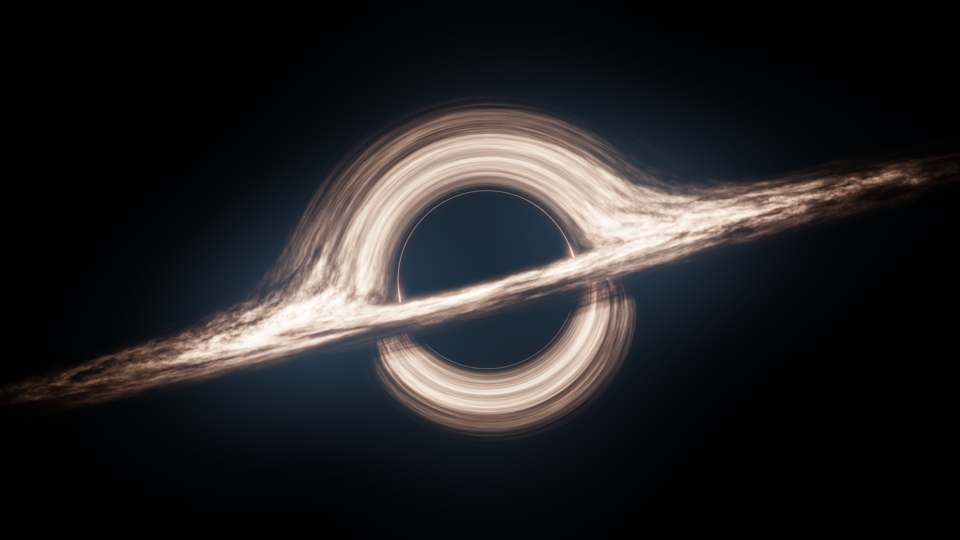
\includegraphics[width=\linewidth]{fig/intro/black-hole.png}
	\caption{
		Computer scientists tend to do badly around black holes.
		\href{https://commons.wikimedia.org/wiki/File:Black_Hole_Full.png}{Illustration}
		by \href{https://commons.wikimedia.org/wiki/User:852278-MCS}{852278-MCS},
		licensed under \href{https://creativecommons.org/licenses/by-sa/4.0/deed.en}{CC BY SA 4.0}.
	}
\end{marginfigure}
Many results of this thesis assume the undecidability of the halting problem:
we hence assume that the reader lives in the familiar spacetime \cite{Hogarth1994NonTuring}.
Should the reader be in rotation around a black hole, we kindly suggest
to them to calmly close this thesis and focus on addressing this situation.

\section*{Acknowledgements}

\todo{todo}